% ===========================================================================
% README_opencode.tex — report on NN-adaptive Bayesian quantum estimation.
% Covers the Ramsey experiment, the estimation problem, the two learned
% policies (TRPO and CEM), and a comparison of their evaluation plots.
% Compile: pdflatex README_opencode.tex
% ===========================================================================

\documentclass[12pt,a4paper]{article}
\usepackage[left=2.00cm,right=2.00cm]{geometry}
\usepackage[T1]{fontenc}
\usepackage[utf8]{inputenc}
\usepackage{float}
\usepackage{caption}
\usepackage{graphicx}
\usepackage{longtable}
\usepackage{subcaption}
\usepackage{amsmath}
\usepackage{hyperref}
\hypersetup{colorlinks=true, linkcolor=blue, urlcolor=blue,
            pdftitle={NN-Adaptive Bayesian Quantum Estimation},
            pdfauthor={Michal Chrzanowski}}
\usepackage{placeins}

% Additions to the supplied preamble:
\usepackage{amssymb}   % \mathbb, \lesssim, \gtrsim
\usepackage{booktabs}  % \toprule/\midrule/\bottomrule, consistent table rules
\usepackage{array}     % >{\raggedright\arraybackslash}p{} column specifications
\usepackage[table]{xcolor} % \cellcolor, shaded table cells
\setlength{\emergencystretch}{2em}   % keeps dense paragraphs within the measure

\graphicspath{{figures/}}

\title{NN-Adaptive Bayesian Quantum Estimation}
\author{Michal Chrzanowski}
\date{\today}

\begin{document}
\maketitle

% ===========================================================================
\section*{Introduction}
% ===========================================================================
The aim of this project was to learn \emph{when} to measure a qubit so that
its frequency is learned as fast as physically possible. The work implements
adaptive Bayesian experimental design for single-qubit Ramsey frequency
estimation: a sequential Monte Carlo filter maintains a posterior over the
unknown Larmor frequency, a policy reads that posterior and chooses the
interrogation time for the next shot, the measurement outcome sharpens the
posterior, and the cycle repeats.

Two policies are trained and compared: \textbf{trust-region policy
optimisation} (TRPO) and the \textbf{cross-entropy method} (CEM). Both were
evaluated over 1.00e+04 held-out frequencies. \textbf{They land in a
statistical tie} --- 2.17e-03 and 2.14e-03 Bayes risk respectively, a 2\%
difference --- despite completely different optimisers. This report explains
the experiment and the estimation problem, describes how each of the two
methods works, and compares their evaluation plots.

\begin{table}[H]
  \centering
  \caption{Abbreviations used in this report.}
  \label{tab:abbreviations}
  \small
  \begin{tabular}{@{}>{\raggedright\arraybackslash}p{0.42\textwidth}
                    >{\raggedright\arraybackslash}p{0.42\textwidth}@{}}
    \toprule
    Full name & Abbreviation \\
    \midrule
    sequential Monte Carlo & SMC \\
    trust-region policy optimisation & TRPO \\
    cross-entropy method & CEM \\
    effective sample size & ESS \\
    reinforcement learning & RL \\
    multilayer perceptron & MLP \\
    Kullback--Leibler divergence & KL \\
    \bottomrule
  \end{tabular}
\end{table}

\noindent\rule{\textwidth}{0.4pt}

% ===========================================================================
\section*{Table of contents}
% ===========================================================================
\begin{itemize}
  \item \hyperref[sec:physics]{The physics}
  \item \hyperref[sec:estimation]{The estimation problem}
  \item \hyperref[sec:configuration]{Parameters}
  \item \hyperref[sec:trpo]{How TRPO works}
  \item \hyperref[sec:cem]{How CEM works}
  \item \hyperref[sec:training]{Training}
  \item \hyperref[sec:evaluation]{Evaluation}
  \item \hyperref[sec:analysis]{Analysis}
  \item \hyperref[sec:summary]{Summary}
\end{itemize}

\noindent\rule{\textwidth}{0.4pt}
\FloatBarrier

% ===========================================================================
\section{The physics}
\label{sec:physics}
% ===========================================================================

% ---------------------------------------------------------------------------
\subsection{The qubit and its state}
\label{sec:qubit-state}
% ---------------------------------------------------------------------------
The system is a single qubit, described by a density matrix $\rho$. The
physically relevant feature of that state is the off-diagonal
\textbf{coherence} $\rho_{01}$, which is what carries the phase accumulated
from the unknown frequency. The qubit is prepared in the equal superposition
$|+\rangle = (|0\rangle + |1\rangle)/\sqrt{2}$, so it starts on the equator
of the Bloch sphere with maximal coherence and equal populations. The
parameter being estimated is the Larmor frequency $\omega$ --- a detuning ---
which sets how fast that phase winds. Dephasing drives the coherence toward
zero without changing the populations, and it is precisely that loss of
coherence which removes information from the state.

% ---------------------------------------------------------------------------
\subsection{The experiment}
\label{sec:the-experiment}
% ---------------------------------------------------------------------------
The experiment is \textbf{Ramsey interferometry} in the presence of pure
dephasing. Each shot runs the same sequence:

\begin{enumerate}
  \item Prepare $|+\rangle = (|0\rangle + |1\rangle)/\sqrt{2}$.
  \item Let the qubit precess freely under
        $H = \tfrac{\omega}{2}\sigma_z$ for a time $t$. This time is the
        \textbf{control variable} --- the one thing the experimenter chooses.
  \item Apply a $\pi/2$ read-out pulse and measure in the computational basis.
  \item Record the binary outcome $d \in \{0, 1\}$.
\end{enumerate}

The qubit is not isolated. Transverse noise destroys the coherence at a rate
set by the coherence time $T_2 = 1.00e+01$,
\begin{equation}
  \rho_{01}(t) = \rho_{01}(0)\,e^{-t/T_2}e^{-i\omega t}.
  \label{eq:coherence}
\end{equation}
Because $\omega$ and $t$ only ever appear as the product $\omega t$, and
$T_2$ shares the units of $t$, units are arbitrary throughout.

% ---------------------------------------------------------------------------
\subsection{The likelihood}
\label{sec:the-likelihood}
% ---------------------------------------------------------------------------
Solving the Lindblad pure-dephasing master equation and applying the Born
rule gives the outcome probability
\begin{align}
  P(d=0 \mid \omega, t)
    &= e^{-t/T_2}\cos^{2}\!\left(\frac{\omega t}{2}\right)
       + \frac{1 - e^{-t/T_2}}{2} \nonumber \\
    &\equiv \frac{1}{2}\bigl[\, 1 + e^{-t/T_2}\cos(\omega t) \,\bigr],
  \label{eq:likelihood}
\end{align}
with $P(d=1 \mid \omega, t) = 1 - P(d=0 \mid \omega, t)$. The two forms are
algebraically identical. The expression reads as a \textbf{decaying
interference fringe}:

\begin{table}[H]
  \centering
  \caption{The likelihood.}
  \label{tab:the-likelihood}
  \small
  \begin{tabular}{@{}>{\raggedright\arraybackslash}p{0.34\textwidth}
                    >{\raggedright\arraybackslash}p{0.56\textwidth}@{}}
    \toprule
    term & meaning \\
    \midrule
    $\cos^{2}(\omega t/2)$ & the Ramsey fringe --- this is what carries
                             information about $\omega$ \\
    $v(t) = e^{-t/T_2}$ & the \textbf{visibility}, or coherent fraction \\
    $(1-v)/2$ & the fully dephased fraction, which returns a coin flip and
                tells you nothing \\
    \bottomrule
  \end{tabular}
\end{table}

As $t \to \infty$ the visibility vanishes, $P(d=0) \to 1/2$, and the
measurement becomes pure noise. \textbf{Decoherence therefore imposes a hard
ceiling on how long it is worth interrogating.} Both the simulator and the
filter use this same expression, and $T_2$ is treated as exactly known: the
model is well specified, with no model mismatch and no nuisance parameter.

% ---------------------------------------------------------------------------
\subsection{Why long interrogation times stop helping}
\label{sec:fisher}
% ---------------------------------------------------------------------------
Differentiating the likelihood gives the single-shot Fisher information
\begin{equation}
  I(\omega; t) = \frac{(\partial_\omega p_0)^{2}}{p_0(1-p_0)}
               = \frac{t^{2} v^{2} \sin^{2}(\omega t)}
                      {1 - v^{2}\cos^{2}(\omega t)},
  \qquad v = e^{-t/T_2}.
  \label{eq:fisher}
\end{equation}
Without decoherence ($v \to 1$) this is just $I = t^2$: information grows
quadratically in interrogation time, which is why longer is better. With
finite $T_2$ the envelope $t^{2}e^{-2t/T_2}$ peaks at $t = T_2$, so the
information per shot is \textbf{bounded} at
$I_{\max} \approx 1.35e-01\,T_2^{2}$. Numerically, for $T_2 = 1.00e+01$ the
optimum sits at $t^{\star} \approx 8.40e+00$--$9.50e+00$, depending on
$\omega$. Beyond $T_2$ the visibility collapses faster than $t^2$ grows, and
additional interrogation time buys nothing.

% ---------------------------------------------------------------------------
\subsection{The competing constraint: phase ambiguity}
\label{sec:phase-ambiguity}
% ---------------------------------------------------------------------------
Fisher information is a \emph{local} quantity, and maximising it is the wrong
move while the prior is still broad. The likelihood depends on $\omega$ only
through $\cos(\omega t)$, which is periodic. Over the prior support
$\Delta\omega = 1.00e+00$ the fringe wraps once $t > 2\pi \approx 6.28e+00$:
several well-separated $\omega$ then produce the same phase, the posterior
goes \textbf{multimodal}, and the filter cannot resolve the aliases.

A good policy must therefore trade off three regimes:

\begin{itemize}
  \item \textbf{small $t$} --- unambiguous, but low information per shot
        ($I \sim t^{2}$);
  \item \textbf{$t \approx T_2$} --- maximum information per shot, but
        aliases a broad prior;
  \item \textbf{$t \gg T_2$} --- decohered, zero information, strictly wasted.
\end{itemize}

The resolution is to grow $t$ \emph{as the posterior narrows}, keeping the
phase spread across the posterior at roughly one radian. An optimal adaptive
policy is therefore expected to show a rising interrogation time as the
posterior collapses.

\noindent\rule{\textwidth}{0.4pt}
\FloatBarrier

% ===========================================================================
\section{The estimation problem}
\label{sec:estimation}
% ===========================================================================

% ---------------------------------------------------------------------------
\subsection{The figure of merit: Bayes risk}
\label{sec:bayes-risk}
% ---------------------------------------------------------------------------
This is a \textbf{Bayesian} estimation problem, and the quantity everything
is judged by is the \textbf{Bayes risk},
\begin{equation}
  r\bigl(h \mid p(\theta)\bigr) = \mathbb{E}_{D_k}\bigl[\,
  \mathrm{tr}\,\mathrm{Cov}(\theta \mid D_k) \,\bigr],
  \label{eq:bayes-risk}
\end{equation}
where $h$ is the experiment-design policy, $D_k = (d_1,\dots,d_k)$ the
measurement record, and smaller is better. It is the risk of the quadratic
loss $L(\hat\theta_k, \theta) = \lVert\hat\theta_k - \theta\rVert_2^{2}$
under the Bayes estimator $\hat\theta_k(D_k) = \mathbb{E}[\theta \mid D_k]$,
that is, the posterior mean. For the single-parameter, experiment-limited
case implemented here, the trace is over a $1\times1$ covariance and the
expectation is estimated by averaging over true $\omega$ values. \textbf{The
Bayes risk is therefore precisely the mean final posterior variance} by which
the methods are ranked below.

% ---------------------------------------------------------------------------
\subsection{The reward and its telescoping identity}
\label{sec:reward}
% ---------------------------------------------------------------------------
The reward is the \textbf{reduction in traced posterior covariance} at each
step,
\begin{align}
  R(D_k) &= \mathrm{tr}\,\mathrm{Cov}(\theta \mid D_{k-1})
            - \mathrm{tr}\,\mathrm{Cov}(\theta \mid D_k) \nonumber \\
         &\xrightarrow{\ d=1\ } V_{k-1} - V_k,
  \label{eq:reward}
\end{align}
with $V_k = \sum_i w_i(\omega_i - \bar\omega)^{2}$. This is not an arbitrary
choice: the negative Bayes risk is the obvious reward but is far too slow to
compute inside a training loop, whereas Eq.~\eqref{eq:reward} is cheap in the
filter framework \emph{and} telescopes to it. For $N$ measurements per
episode,
\begin{equation}
  \mathbb{E}_{D_N}\left[\sum_{j=1}^{N} R(D_j)\right]
    = \mathrm{const} - r\bigl(h \mid p(\theta)\bigr),
  \qquad \mathrm{const} = \mathrm{tr}\,\mathrm{Cov}(\theta).
  \label{eq:telescope}
\end{equation}
So maximising the episode return \textbf{provably minimises the Bayes
risk} --- provided the return is undiscounted.

% ---------------------------------------------------------------------------
\subsection{The inference layer: the particle filter}
\label{sec:particle-filter}
% ---------------------------------------------------------------------------
$\omega$ is a \textbf{static} parameter --- it does not evolve --- so the
filter only ever reweights particles; the particle locations move solely
during resampling. The posterior is represented by $N$ particles
$\{\omega_i\}$ with log-weights $\{\log w_i\}$, updated in the log domain,
\begin{equation}
  \log w_i \leftarrow \log w_i + \log P(d \mid \omega_i, t)
                    - \mathrm{logsumexp}(\cdot),
  \label{eq:bayes-update}
\end{equation}
and renormalised every step. The filter's health is monitored by the Kish
effective sample size $\mathrm{ESS} = 1/\sum_i w_i^{2} \in [1, N]$.

Resampling fires when $\mathrm{ESS} < 7.50e-01\,N$, an aggressive threshold,
so it triggers on most steps. The scheme used throughout is \textbf{Liu--West
kernel resampling} ($a = 9.80e-01$),
\begin{equation}
  \omega_i' = a\,\omega_{\mathrm{idx}(i)} + (1-a)\,\bar{\omega}
              + \varepsilon_i,
  \qquad \varepsilon_i \sim \mathcal{N}\bigl(0,\, h^{2}\Sigma\bigr),
  \quad h^{2} = 1 - a^{2}.
  \label{eq:liu-west}
\end{equation}
The shrinkage toward the weighted mean exactly cancels the variance added by
the jitter ($a^{2}\Sigma + h^{2}\Sigma = \Sigma$), so the posterior's first
two moments are preserved. The jitter is what prevents particle
impoverishment: a static parameter is never diffused by process noise, so
plain multinomial resampling would collapse all particles onto a handful of
duplicated values.

% ---------------------------------------------------------------------------
\subsection{The control problem}
\label{sec:control-problem}
% ---------------------------------------------------------------------------
The control problem is framed as a standard sequential decision problem:

\begin{table}[H]
  \centering
  \caption{The control problem.}
  \label{tab:the-control-problem}
  \small
  \begin{tabular}{@{}>{\raggedright\arraybackslash}p{0.20\textwidth}
                    >{\raggedright\arraybackslash}p{0.70\textwidth}@{}}
    \toprule
    component & definition \\
    \midrule
    observation & posterior mean, posterior variance, and the last
                  3.00e+01 interrogation times ($3.20e+01$ inputs) \\
    action & interrogation time $t \in [1.00e-01,\, 3.00e+03]$ \\
    reward & $V_{k-1} - V_k$ \\
    episode & 1.00e+02 measurements (training) / 1.25e+02 (evaluation),
              one true $\omega$ per episode \\
    \bottomrule
  \end{tabular}
\end{table}

\noindent\rule{\textwidth}{0.4pt}
\FloatBarrier

% ===========================================================================
\section{Parameters}
\label{sec:configuration}
% ===========================================================================
A single parameter set is shared by everything, so all comparisons are
apples-to-apples.

\begin{table}[H]
  \centering
  \caption{Parameters.}
  \label{tab:parameters}
  \small
  \begin{tabular}{@{}>{\raggedright\arraybackslash}p{0.22\textwidth}
                    >{\raggedright\arraybackslash}p{0.30\textwidth}
                    >{\raggedright\arraybackslash}p{0.38\textwidth}@{}}
    \toprule
    symbol & value & meaning \\
    \midrule
    $\omega$ (prior) & $\mathrm{Uniform}(0, 1)$,
                       $\mathrm{Var}[\omega] = 8.33e-02$
                     & unknown Larmor frequency / detuning \\
    $T_2$ & 1.00e+01 & transverse coherence time \\
    $t$ (control) & $[1.00e-01,\, 3.00e+03]$ & interrogation time chosen per shot \\
    episode length & 1.00e+02 / 1.25e+02 & measurements per episode (train / eval) \\
    particles & 2.00e+03 & SMC particles (training and evaluation) \\
    evaluation set & 1.00e+04 & true $\omega$ values \\
    discount factor & 9.90e-01 & TRPO reward discount \\
    resample threshold & 7.50e-01$N$ & ESS below which resampling fires \\
    Liu--West shrinkage & 9.80e-01 & kernel parameter $a$ \\
    target KL & 1.00e-02 & TRPO trust-region budget \\
    \bottomrule
  \end{tabular}
\end{table}

\noindent With $\omega \lesssim 1.00e+00$ and $T_2 = 1.00e+01$, roughly
$\omega T_2 \lesssim 1.00e+01$ radians of phase accumulate before coherence
is lost, so a few fringes are resolvable within the coherence window. Over
the prior support the fringe first wraps at
$t = 2\pi \approx 6.28e+00$, which sets the boundary between the
aliasing-safe and aliasing-prone regimes.

\noindent\rule{\textwidth}{0.4pt}
\FloatBarrier

% ===========================================================================
\section{How TRPO works}
\label{sec:trpo}
% ===========================================================================
\textbf{TRPO} is a policy-gradient method. At each update it maximises a
linear surrogate of the expected return while constraining the
Kullback--Leibler divergence between the old and the new policy to a trust
region. Bounding the step size is what keeps the method stable: a single
update cannot move the policy arbitrarily far, which matters because the
control problem is non-stationary as the posterior evolves. A separately
trained value function supplies a baseline that reduces the variance of the
advantage estimate used in the surrogate.

In this implementation both the policy and the value function are
multilayer perceptrons with two hidden layers of 2.56e+02 units each. The
actor is an unbounded Gaussian; its sampled action is clipped to the allowed
interrogation-time interval inside the environment step. The policy is
trained \textbf{from scratch}, with no supervised initialisation; the
training procedure and its scale are given in
\hyperref[sec:training]{Training}.

% ===========================================================================
\section{How CEM works}
\label{sec:cem}
% ===========================================================================
\textbf{CEM} is a gradient-free evolutionary search. It maintains a Gaussian
distribution over a flat parameter vector, samples a population from it,
evaluates every member of the population on the task, keeps the best elite
fraction, and refits the distribution to those elites. Iterating this
concentrates the search distribution on high-return parameters without ever
computing a gradient.

Here the parameter vector is the flattened 5.45e+02-dimensional weight
vector of a small policy network with one hidden layer of 1.60e+01 units and
a hyperbolic-tangent activation. Its output is squashed by a sigmoid,
\begin{equation}
  t = t_{\min} + (t_{\max} - t_{\min})\,\sigma(z),
  \label{eq:cem-output}
\end{equation}
so the network can never emit an out-of-range interrogation time --- the
action bound is structural rather than clipped after the fact. The training
procedure and its scale are given in
\hyperref[sec:training]{Training}.

\noindent\rule{\textwidth}{0.4pt}
\FloatBarrier

% ===========================================================================
\section{Training}
\label{sec:training}
% ===========================================================================
Both policies are trained in the same environment. Each episode draws one
true frequency $\omega \sim \mathrm{Uniform}(0, 1)$ and runs for
1.00e+02 measurements. The posterior is maintained by the particle filter
with 2.00e+03 particles, and at every step the agent observes the posterior
mean, the posterior variance and the last 3.00e+01 interrogation times
(3.20e+01 inputs), and receives the reward $V_{k-1} - V_k$. The discount
factor is 9.90e-01.

\textbf{TRPO.} The policy is trained \textbf{from scratch}, with no
supervised initialisation, for 1.00e+05 episodes --- 1.00e+07 timesteps ---
with a target KL of 1.00e-02. Checkpoints are written every 5.00e+04 steps,
so a partially trained policy can be evaluated at any point and a crash costs
at most one interval. A full run takes \textbf{2 h 24 m} on CPU.

\textbf{CEM.} The gradient-free search uses a population of 1.00e+03, an
elite fraction of 1.00e-01 and 1.00e+02 generations, with 2.00e+03 particles
and 1.00e+02-step episodes. The returned policy is the mean of the final
search distribution. A full run takes \textbf{54 minutes} on CPU.

Both runs log their per-episode (TRPO) or per-generation (CEM) metrics and
their checkpoints to MLflow.

\noindent\rule{\textwidth}{0.4pt}
\FloatBarrier

% ===========================================================================
\section{Evaluation}
\label{sec:evaluation}
% ===========================================================================
The trained policies are evaluated on the NumPy reference harness, which
runs at float64 one frequency at a time. Evaluation uses 1.00e+04 held-out
frequencies, drawn independently of the training draw; 1.25e+02 measurements
per episode; 2.00e+03 particles; Liu--West resampling; and
$T_2 = 1.00e+01$. The figure of merit is the Bayes risk of
Eq.~\eqref{eq:bayes-risk}, which for this single-parameter,
experiment-limited problem is exactly the mean final posterior variance
averaged over the 1.00e+04 frequencies. Lower is better. The analysis below
reports this quantity.

\noindent\rule{\textwidth}{0.4pt}
\FloatBarrier

% ===========================================================================
\section{Analysis}
\label{sec:analysis}
% ===========================================================================
Table~\ref{tab:comparison} gives the headline numbers over the 1.00e+04
held-out frequencies. Lower Bayes risk is better.

\begin{table}[H]
  \centering
  \caption{TRPO and CEM over 1.00e+04 held-out frequencies.}
  \label{tab:comparison}
  \small
  \begin{tabular}{@{}>{\raggedright\arraybackslash}p{0.34\textwidth}
                    >{\raggedright\arraybackslash}p{0.27\textwidth}
                    >{\raggedright\arraybackslash}p{0.27\textwidth}@{}}
    \toprule
    quantity & TRPO & CEM \\
    \midrule
    training & 1.00e+05 episodes, 1.00e+07 timesteps, 2 h 24 m
             & 1.00e+02 generations $\times$ 1.00e+03 population, 54 min \\
    \textbf{Bayes risk over 1.00e+04 $\omega$} & \textbf{2.17e-03} & \textbf{2.14e-03} \\
    mean $t$ & 4.00 & 6.67 \\
    min / max $t$ & 0.10 / 9.85 & 2.16 / 15.60 \\
    final ESS (of 2.00e+03) & 1960 & 1904 \\
    \bottomrule
  \end{tabular}
\end{table}

The two methods land in a \textbf{statistical tie} --- 2.17e-03 against
2.14e-03, a 2\% difference --- despite completely different optimisers and
very different chosen times: CEM settles on interrogation times roughly
1.7$\times$ longer than TRPO's, and never goes below $t = 2.16$, where TRPO
ranges down to the action floor.

% ---------------------------------------------------------------------------
\subsection{Posterior averaged over omegas}
\label{sec:posterior-averaged-over-omegas}
% ---------------------------------------------------------------------------
Mean posterior variance across all 1.00e+04 $\omega$. Both policies fall from
the prior's 8.33e-02 to about 2.10e-03 and flatten out well before the
1.25e+02nd measurement.

\begin{figure}[H]
  \centering
  \begin{subfigure}[t]{0.48\textwidth}
    \centering
    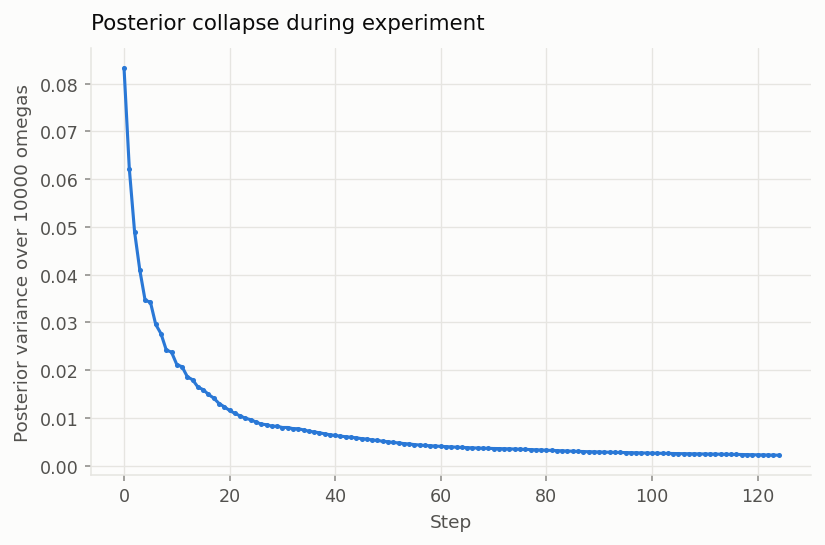
\includegraphics[width=\textwidth]{trpo_posterior_variance_over_omega}
    \caption{TRPO}
    \label{fig:posterior-collapse-trpo}
  \end{subfigure}\hfill
  \begin{subfigure}[t]{0.48\textwidth}
    \centering
    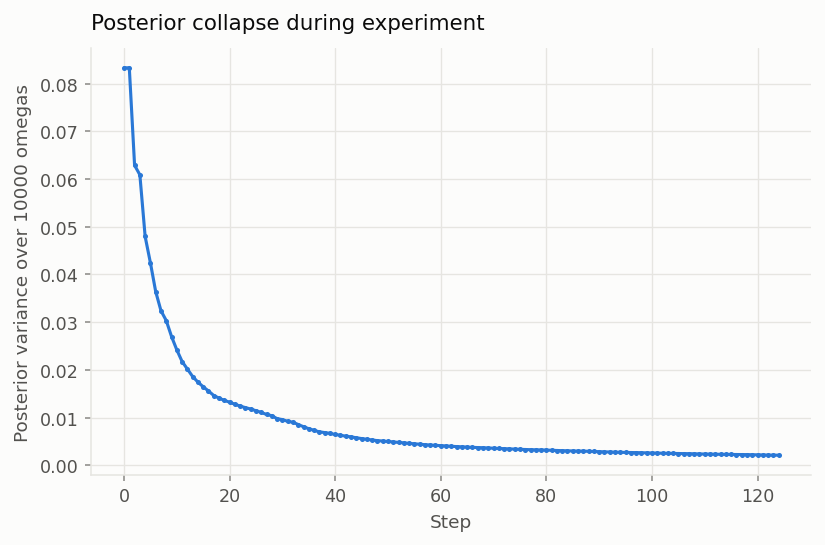
\includegraphics[width=\textwidth]{cem_posterior_variance_over_omega}
    \caption{CEM}
    \label{fig:posterior-collapse-cem}
  \end{subfigure}
  \caption{Posterior averaged over omegas for TRPO and CEM.}
  \label{fig:posterior-collapse}
\end{figure}

\noindent\rule{\textwidth}{0.4pt}
\FloatBarrier

% ===========================================================================
\section{Summary}
\label{sec:summary}
% ===========================================================================
This project implements adaptive Bayesian frequency estimation for a single
qubit, with a sequential Monte Carlo filter tracking the posterior and a
learned policy choosing the interrogation time at each shot. The physics and
the estimation machinery are in place and behave: the likelihood, the
Bayes-risk figure of merit, the variance-reduction reward and its
telescoping identity all hold.

Two learned policies were trained and compared. TRPO and CEM land in a
statistical tie over 1.00e+04 held-out frequencies, at 2.17e-03 and 2.14e-03
Bayes risk respectively --- a 2\% difference. Averaged over those
frequencies, the posterior variance falls from the prior's 8.33e-02 to about
2.10e-03 for both policies and flattens out well before the end of the
episode.

\section*{References}

D.~Fiderer, J.~Schuff, and D.~Braun, \emph{Neural-network heuristics for
adaptive Bayesian quantum estimation}, PRX Quantum \textbf{2}, 020303
(2021); preprint dated 2020-03-05.

\end{document}